\documentclass[prb,preprint]{revtex4-1} 
% The line above defines the type of LaTeX document.
% Note that AJP uses the same style as Phys. Rev. B (prb).

\usepackage{amsmath}  % needed for \tfrac, \bmatrix, etc.
\usepackage{amsfonts} % needed for bold Greek, Fraktur, and blackboard bold
\usepackage{graphicx} % needed for figures
\usepackage{tabularx}

\begin{document}

\title{Superconductivity}
% In a long title you can use \\ to force a line break at a certain location.

\author{Jiajun Shi}
\email{jshi15@amherst.edu} 
\affiliation{Department of Physics, Smith College, Northampton, MA 01063}
\author{He Claudia Yun}
\email{hyun@smith.edu}
\affiliation{Department of Physics, Smith College, Northampton, MA 01063}

% See the REVTeX documentation for more examples of author and affiliation lists.

\date{\today}

%____________abstract____________________________________________

\begin{abstract}

\end{abstract}

\maketitle 

%____________Introduction____________________________________________
\section{Introduction}

%____________Experiment____________________________________________
\section{Experiment}
Temperature and resistance are measured for two different materials: $YBa_{2}Cu_{3}O_{7}$ (YBCO) and $Bi_{2}Sr{2}Ca_{2}Cu_{3}O_{9}$ (BISCO). The experiments are done in two different ways for different materials.\\
\subsection{YBCO}
The setup of YBCO experiment is shown in the Fig. \ref{setup}. The device (Fig. \ref{sample}), including the sample, a thermocouple, a current probe and a voltage probe, is put in a plastic-foam cup and immersed in sands, which serve as insulator. %And the leads from the device are connected to a power supply and two digital multimeters (Fig. \ref{meters}) as shown in Fig. \ref{connection}.

\begin{figure}[h]
\centering
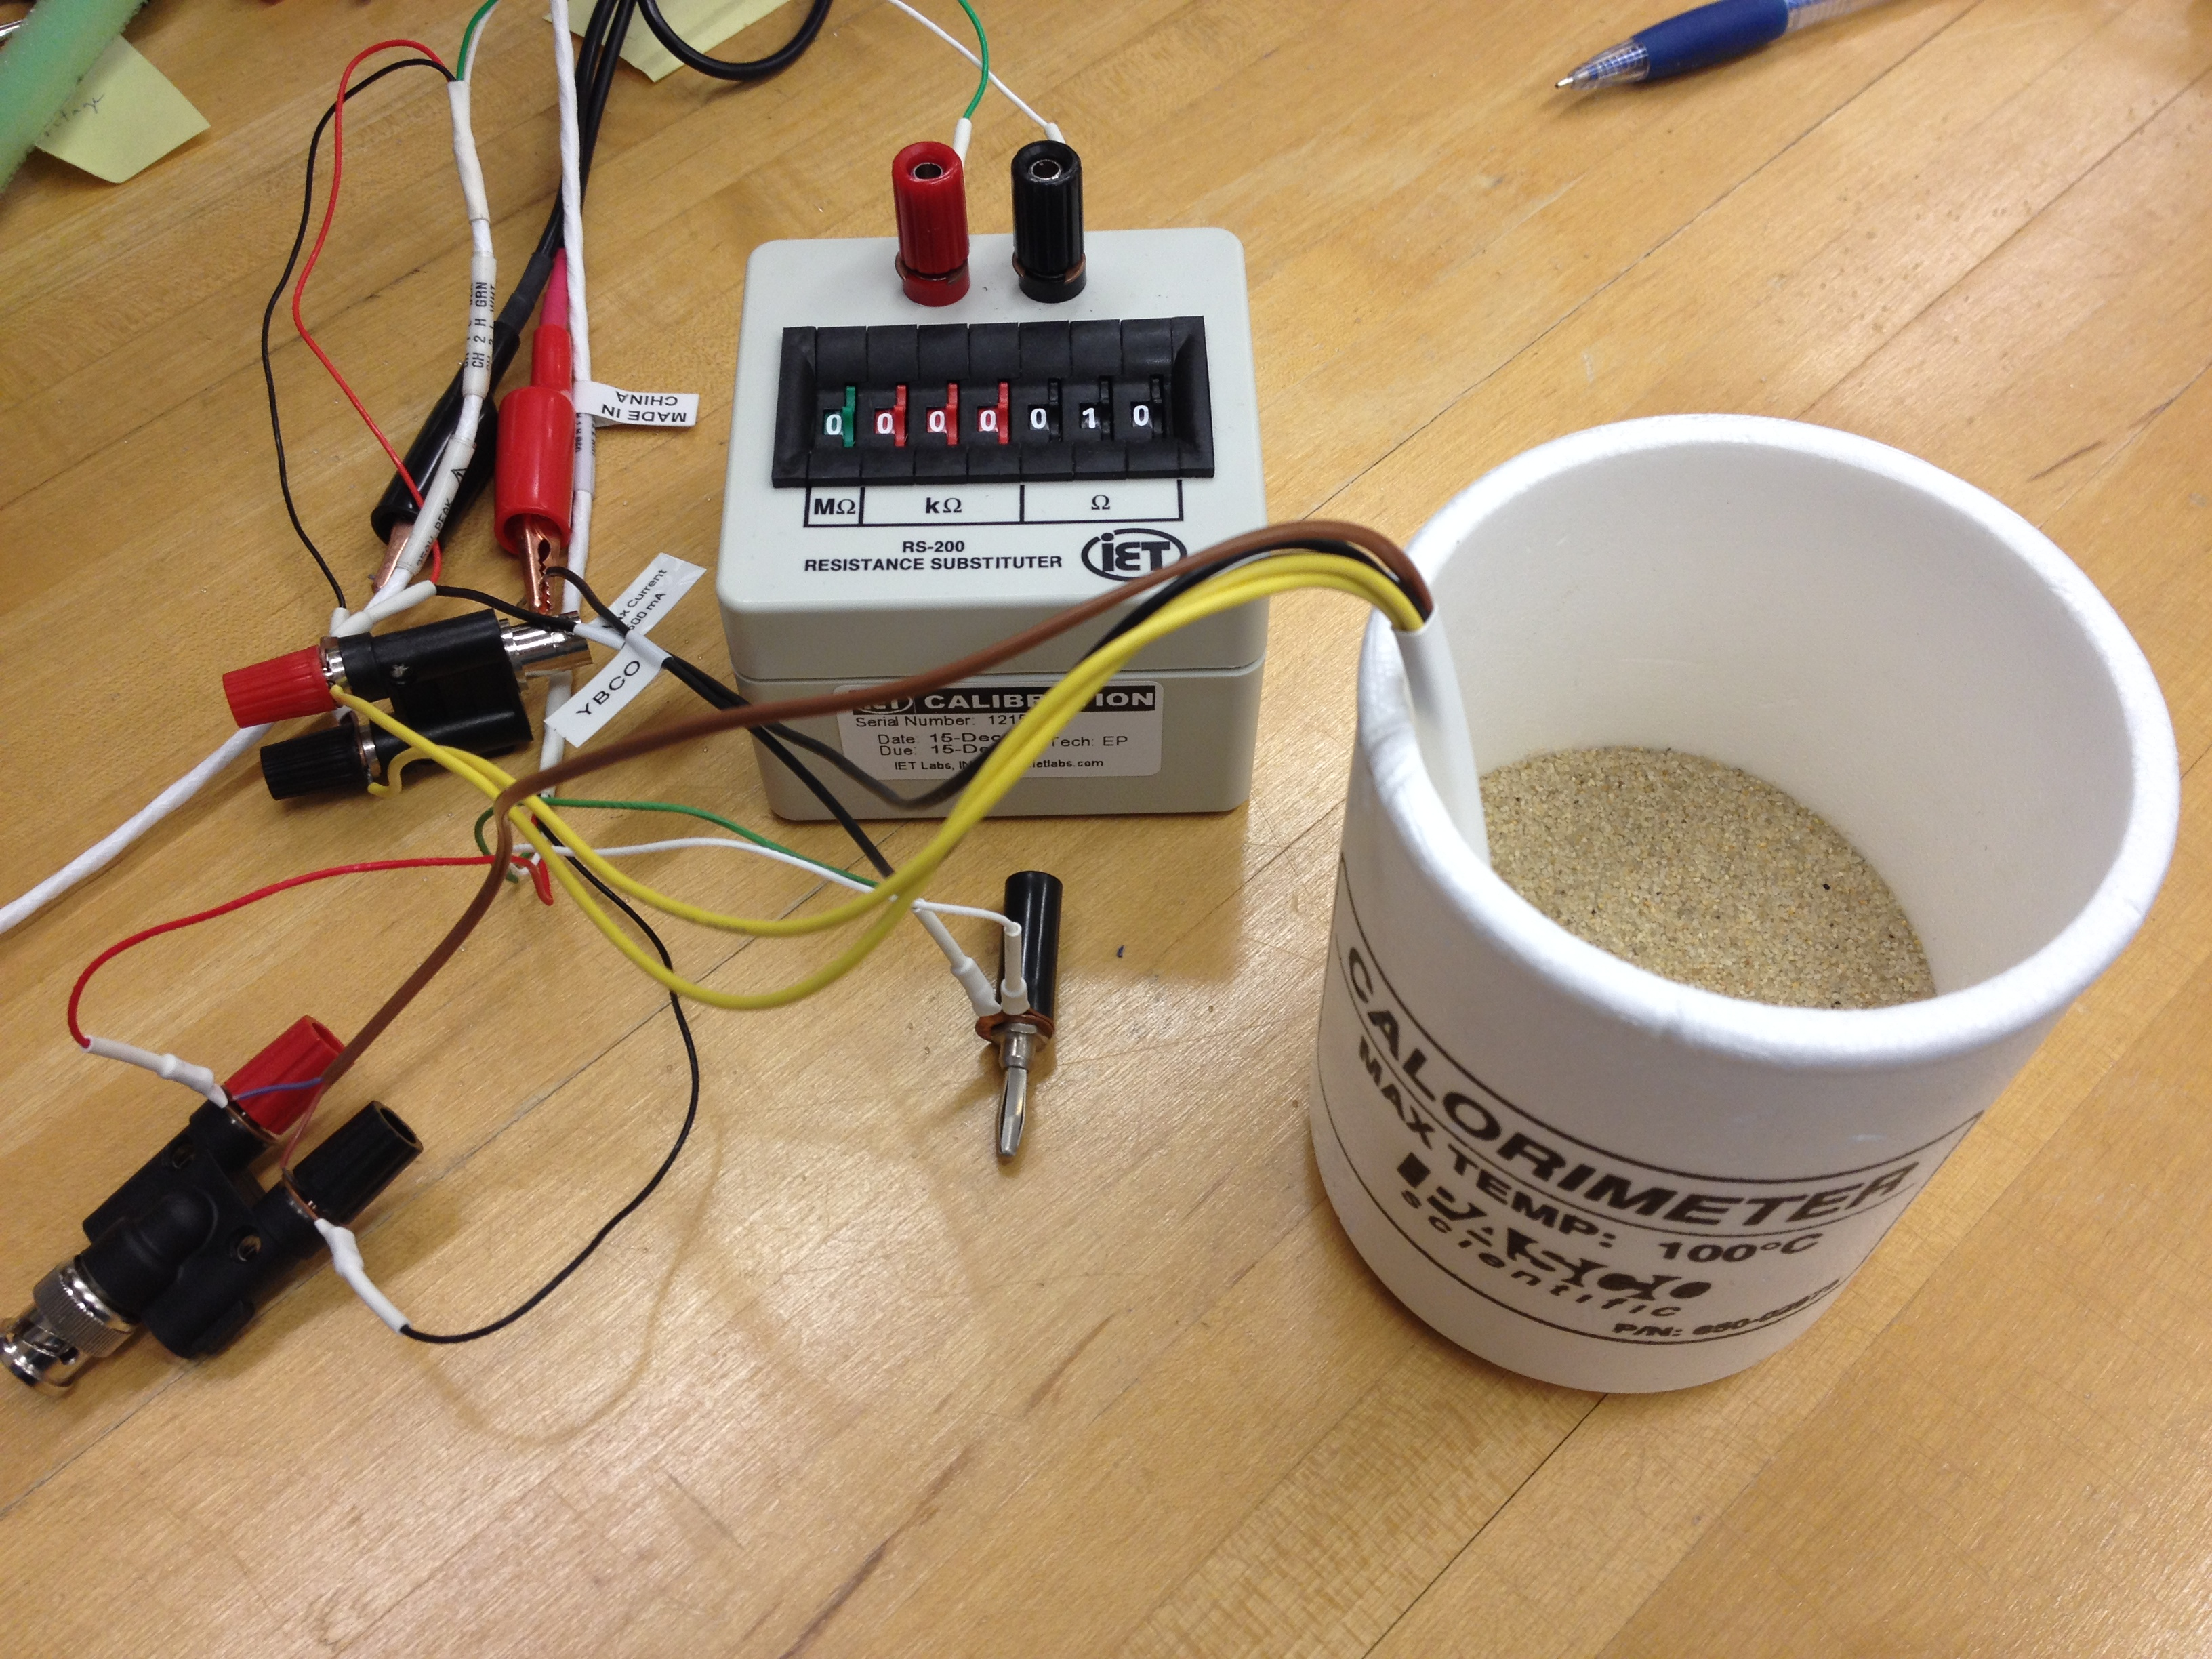
\includegraphics[width=16cm]{ybcosetup.jpg}
\caption{Picture of the experiment setup}
\label{setup}
\end{figure}

\begin{figure}[h]
\centering
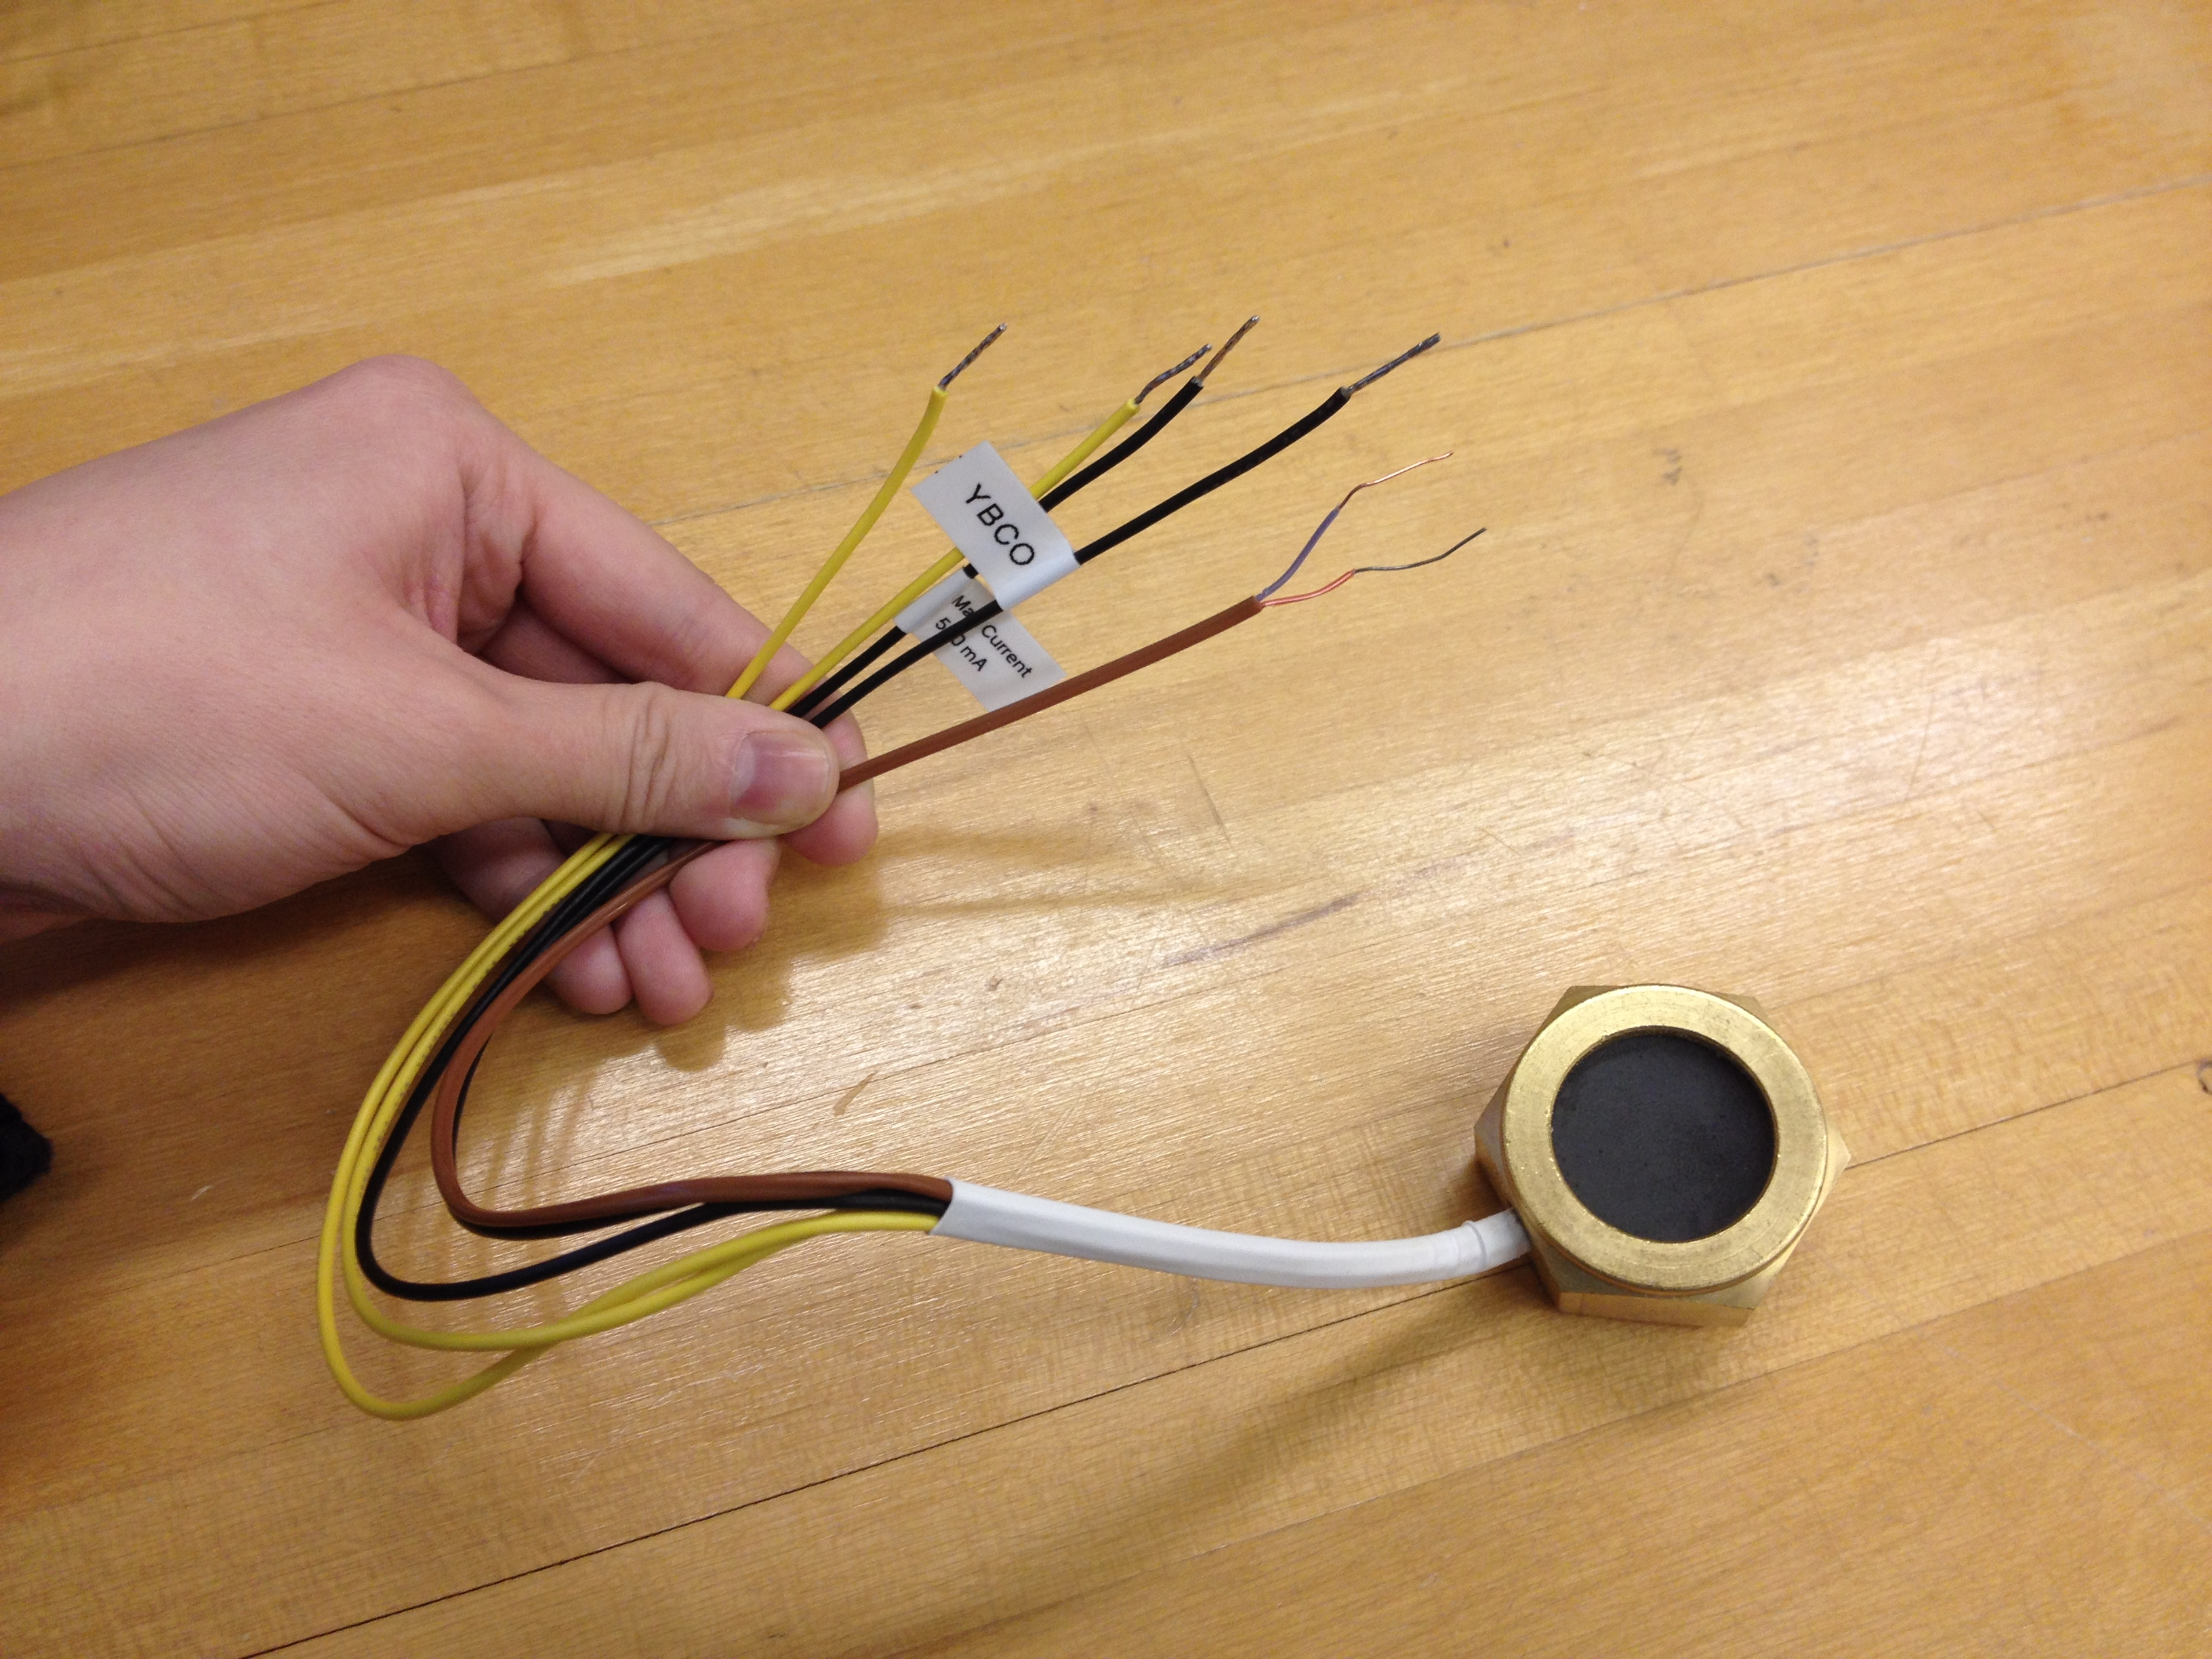
\includegraphics[width=16cm]{ybcosample.jpg}
\caption{Picture of the device, including YBCO sample (the black disk on top), thermocouple (brown lead), current (black leads) and voltage probes (yellow leads)}
\label{sample}
\end{figure}

The device has 

\begin{figure}[h]
\centering
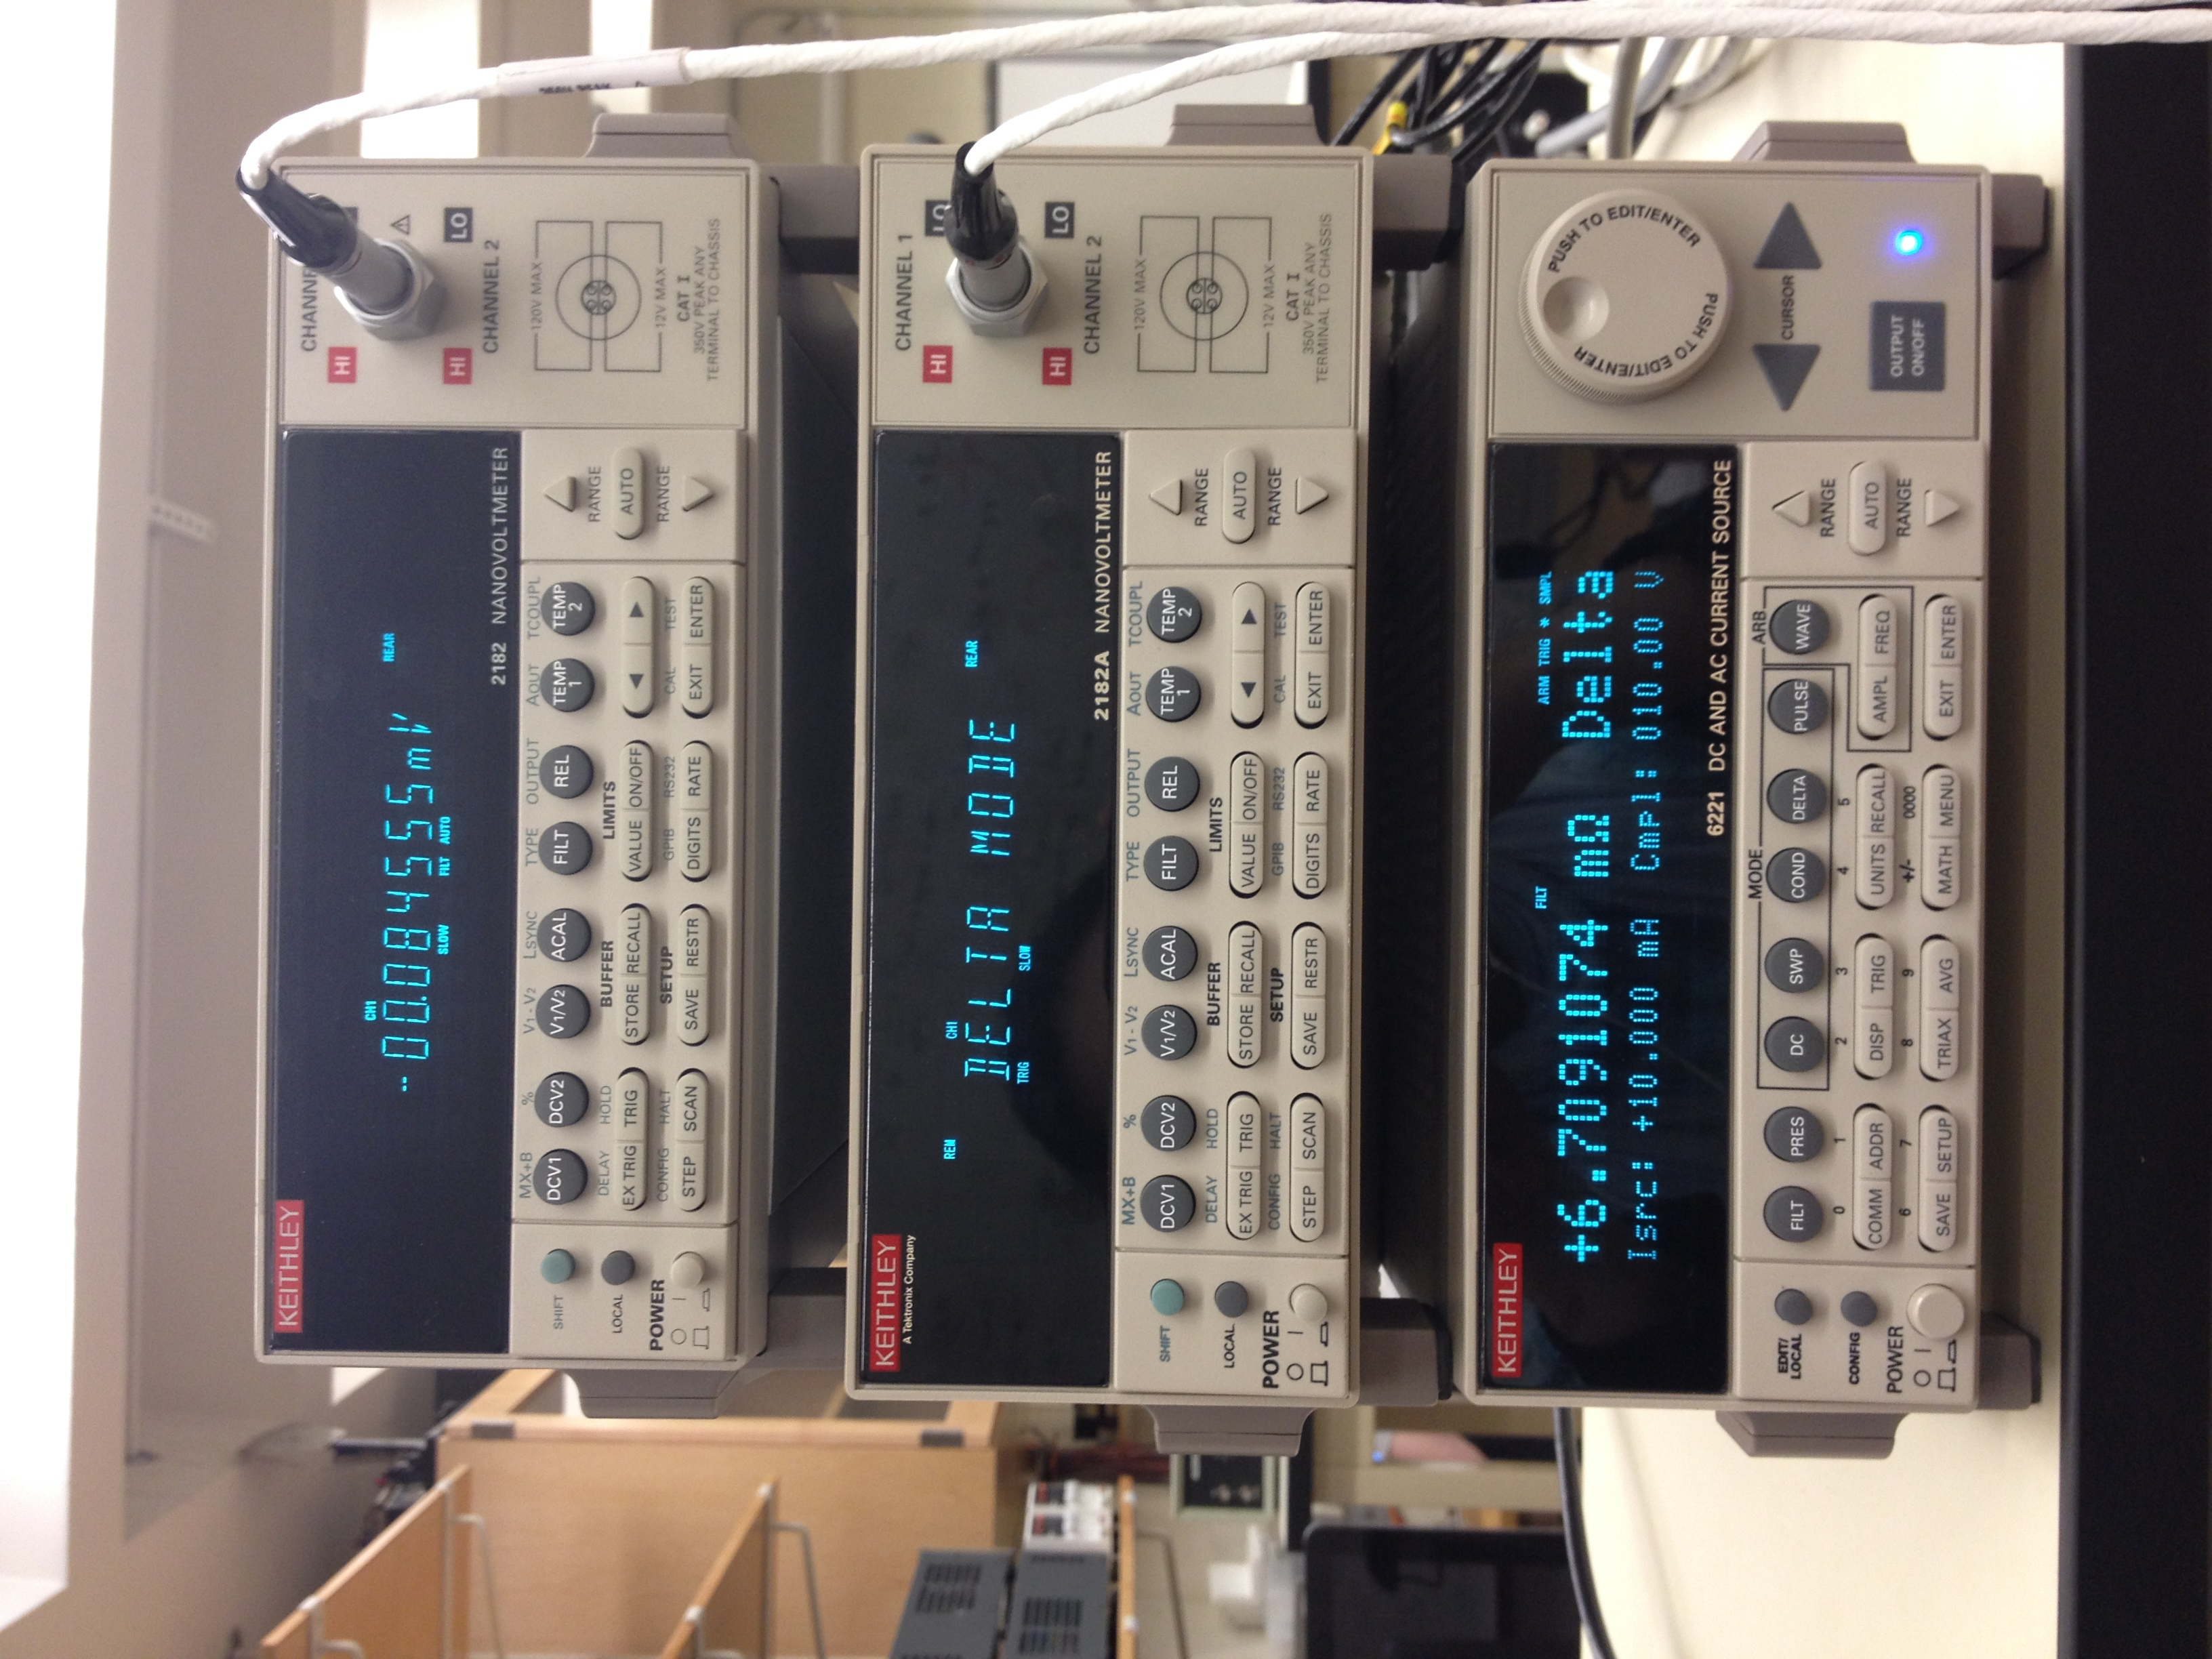
\includegraphics[width=16cm]{ybcometers.jpg}
\caption{The three digital meters used. The top one measures the voltage of the thermocouple, the middle one ? and the bottom one is a power source that is in delta mode, and it reads the resistance of the YBCO sample.}
\label{meters}
\end{figure}

%\begin{figure}[h]
%\centering
%\includegraphics[width=16cm]{connection.jpg}
%\caption{Schematic of how the device is connected to the power supply and the meters}
%\label{connection}
%\end{figure}




\subsection{BISCO}


%____________Results____________________________________________
\section{Results}



%____________Discussion____________________________________________
\section{Discussion}

%____________Conclusion____________________________________________
\section{Conclusion}


\begin{acknowledgments}

We gratefully acknowledge Nathanael Fortune and Dana Parsons, who helped with the experimentation and editing of this experiment.  This work was supported by the Smith College Physics Department.

\end{acknowledgments}


\begin{thebibliography}{99}

%\bibitem{wik} Double Slit Experiment, \url{<http://upload.wikimedia.org/wikipedia/commons/c/c2/Single_slit_and_double_slit2.jpg/>}.
\bibitem{drawcircuit} Scheme-it, http://www.digikey.com/schemeit
\bibitem{energy} Optical Pumping, http://internal.physics.uwa.edu.au/~stamps/2006Y3Lab/SteveAndBlake/theoretical.html

\end{thebibliography}

%\newpage   % Start a new page for tables

\end{document}
